\chapter{Stand der Technik}
\label{Kap2}
\label{chap:Kap2}

Im folgenden Kapitel werden verwandte Arbeiten und Applikationen zum Thema sowie Technisches Grundlagenwissen, das zur Umsetzung der Interaktion benötigt wird, beschrieben.

\section{Grundlagen zum gestenbasierten Transfer von Daten}

Die Nutzung einer gestenbasierten Interaktion zum Datenaustausch wurde schon von einigen wissenschaftlichen Arbeiten behandelt und in Applikationen umgesetzt. An dieser Stelle wird eine Auswahl an Arbeiten und Applikationen vorgestellt die Ähnlichkeit mit der geplanten Bump-Interaktion aufweisen.

\textbf{Hinckley} \cite{Hinckley:2003:SGM:964696.964713} beschreibt eine Interaktion, mit der Tablet-Computer über eine Bump-Interaktion miteinander verbunden werden. Das anstoßen der Geräte aneinander (Siehe Abbildung \ref{fig:hinckley}) baut eine Verbindung zwischen den Geräten auf, indem die generierten Accelerometer Daten zusammen mit einem Timestamp über ein lokales WLAN-Netzwerk ausgetauscht und abgeglichen werden. Die Bump-Interaktion entwickelt Hinckley auf der Metapher des Anstoßens von zwei Trinkgläsern aneinander. Deshalb führt er die Trinkgläser-Metapher auch für den Datenaustausch fort und definiert eine Geste, die dem umschütten von Flüssigkeit aus einem Glas in ein anderes entspricht. Dieser Metapher folgend, schüttet eines der Geräte ausgewählte Daten durch eine drehende Bewegung in das andere Gerät (Siehe Abbildung \ref{fig:hinckley2}).

\begin{figure}[H]
\begin{minipage}[h]{7cm}
	\centering
	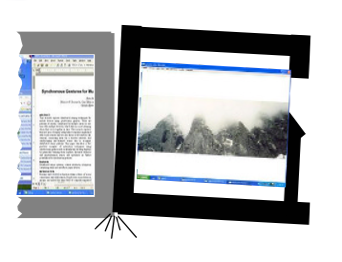
\includegraphics[width=5cm]{kapitel2/hinkley.png}
	\caption{Bump Tablet-Computer \cite{Hinckley:2003:SGM:964696.964713}}
	\label{fig:hinckley}
\end{minipage}
\hfill
\begin{minipage}[h]{7cm}
	\centering
	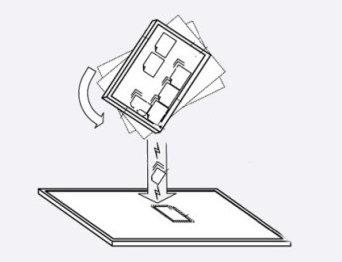
\includegraphics[width=5cm]{kapitel2/hinkley2.png}
	\caption{Daten ausschütten \cite{HinkleyPic2:Online}}
	\label{fig:hinckley2}
\end{minipage}
\end{figure}


Ähnlich wie bei Hinckley werden bei der Applikation \textbf{Bump} \cite{Bump:Online} die Beschleunigungssensoren von Smartphones und Tablets genutzt um Bump-Events festzustellen (Siehe Abbildung \ref{fig:bumpPhone}). Die Applikation sendet, nachdem ein Bump festgestellt wurde, die ausgewählten Nutzdaten, sowie Charakteristiken des Bumps an einen Server. Der Sever erkennt eingehende Bumps durch einen Algorithmus und ordnet Bump-Partner basierend auf den Charakteristiken der Bumps einander zu. Der Algorithmus nutzt unter anderem GPS-Standortdaten, um die Anzahl der möglichen Treffer zu reduzieren, sowie eine Anzahl anderer Daten, um die richtigen Bump-Partner zu identifizieren. Nachdem der Server die Geräte einander zugeordnet hat, leitet er die entsprechenden Nutzdaten an die jeweiligen Geräte weiter. Der Datenaustausch zwischen mobilen Endgeräten und Computern ist auch möglich. Dazu muss das mobile Gerät auf die Leertaste der Computertastatur gebumped werden (Siehe Abbildung \ref{fig:bumpPC}).

\begin{figure}[H]
\begin{minipage}[h]{7cm}
	\centering
	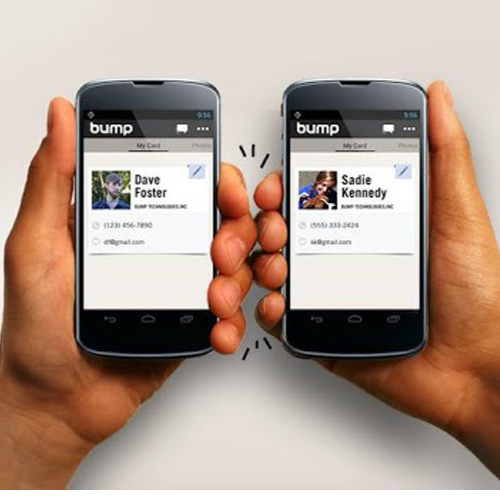
\includegraphics[width=5.5cm]{kapitel2/bumpPhone.png}
	\caption{Bump-Geste Smartphones \cite{BumpPicPhone:Online}}
	\label{fig:bumpPhone}
\end{minipage}
\hfill
\begin{minipage}[h]{7cm}
	\centering
	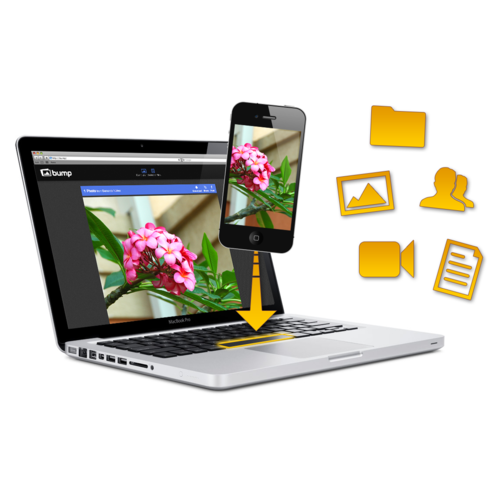
\includegraphics[width=5.5cm]{kapitel2/bumpPC.png}
	\caption{Bump-Geste PC \cite{Bump:Online}}
	\label{fig:bumpPC}
\end{minipage}
\end{figure}

\textbf{Yatani et al.} \cite{Yatani:2006:TII:1184855.1184874} nutzen Accelerometer Daten um Wurf- und Schwung-Gesten zu erkennen. Mit einer Wurf-Geste werden Daten, zu einem einzelnen Empfänger geworfen. Durch eine Schwung Geste können mehrere Geräte auf einmal als Empfänger ausgewählt werden. Der Datenaustausch erfolgt über einen Server in einem lokalen \acs{WLAN}-Netzwerk. Der Server ist ebenfalls dafür zuständig, die Position und Orientierung der Geräte zu verarbeiten, um so Sender und Empfänger einander zuzuordnen. Für die Positionsbestimmung wird ein speziell entwickeltes System genutzt, mit dem die Position und Orientierung der Endgeräte über eine Kamera erkannt wird.

\begin{figure}[H]
\begin{minipage}[h]{7cm}
	\centering
	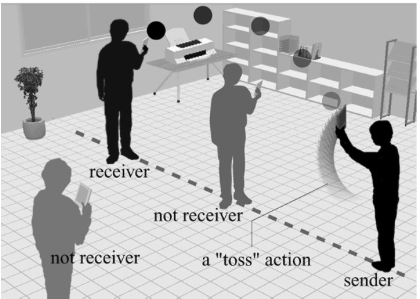
\includegraphics[width=5.5cm]{kapitel2/yatani1.png}
	\caption{Wurf- und Fang-Geste \cite{Yatani:2006:TII:1184855.1184874}}
	\label{fig:yatani1}
\end{minipage}
\hfill
\begin{minipage}[h]{7cm}
	\centering
	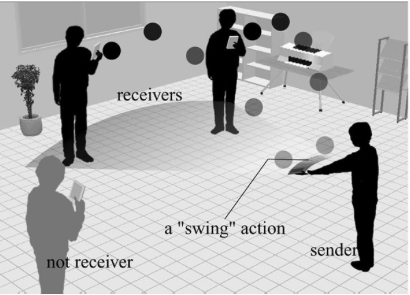
\includegraphics[width=5.5cm]{kapitel2/yatani2.png}
	\caption{Schwung-Geste \cite{Yatani:2006:TII:1184855.1184874}}
	\label{fig:yatani2}
\end{minipage}
\end{figure}

\textbf{Hoccer} ist eine Applikation, die über zwei Gesten verfügt, mit denen Daten zwischen Endgeräten ausgetauscht werden können. Zum einen gibt es die Swipe Geste (Siehe Abbildung \ref{fig:hocSwipe}) und zum anderen eine Wurf und Fang Geste, die vergleichbar mit der Geste von Yatani et al. ist. Mit der Swipe Geste wird über den Touchscreen eine geöffnete Datei von einem Gerät auf das andere geschoben. Bei der Wurf und Fang Geste, führt ein Anwender die Wurf Geste aus und wirft einem zweiten Anwender die Daten, wie mit einem Frisbee, zu. Dieser muss sich als Empfänger identifizieren indem er sein Endgerät nach oben hält, als wollte er das Frisbee fangen. Die Applikation funktioniert technisch ähnlich wie Bump über \acs{GPS}-Standortdaten mit einem Server, der Geräte zuordnet und den Datenverkehr zwischen den Geräten steuert. \cite{Hoccer:Online}

\begin{figure}[H]
	\centering
	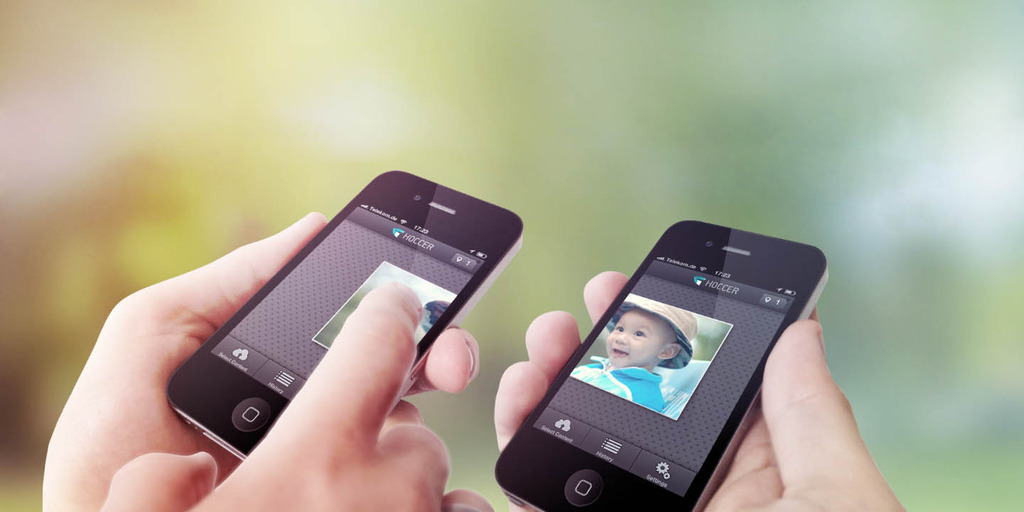
\includegraphics[width=8cm]{kapitel2/hoccerSwipe.jpg}
	\caption{Hoccer Swipe-Geste \cite{HoccerPics:Online}}
	\label{fig:hocSwipe}
\end{figure}

\paragraph{Lucero et al.} \cite{Lucero:2011:PCU:1978942.1979201} haben ein Gesten-gesteuertes System entwickelt, mit dem eine Gruppe von Personen ihre auf Smartphones gespeicherten Photosammlungen durchblättern und untereinander Photos austauschen können. Dazu müssen die Smartphones aller Anwender zusammen auf einem Tisch liegen, am besten in einem Kreis angeordnet. Mit der Hilfe von Gesten kann jeder Anwender durch seine individuelle Photosammlung blättern. Dazu muss er das Smartphone rechts kippen um ein Photo weiterzublättern (Siehe Abbildung \ref{fig:passtThem1}) oder nach links kippen um zurückzublättern. Durch einen Tap auf den Touchscreen rechts oder links kann auch entsprechend vor oder zurückgeblättert werden. Möchte ein Anwender ein einzelnes Bild teilen, muss er so lange die Tap-Geste auf dem Touchscreen ausführen bis eine Miniaturansicht des ausgewählten Photos erscheint. Dieses Bild kann anschließend durch eine Swipe-Geste in die Richtung des Zielgeräts auf dieses übertragen werden. Das System nutzt Accelerometer Daten, um die Geste zum weiterblättern zu erkennen und tauscht die Daten zwischen den Geräten über ein WLAN Netzwerk aus. Für die Identifizierung des Zielgeräts beim Datenaustausch wurde ein spezielles Multi-Emitter Tracking System verwendet, mit dem die Position der Endgeräte festgestellt werden kann.

\begin{figure}[H]
\begin{minipage}[h]{7cm}
	\centering
	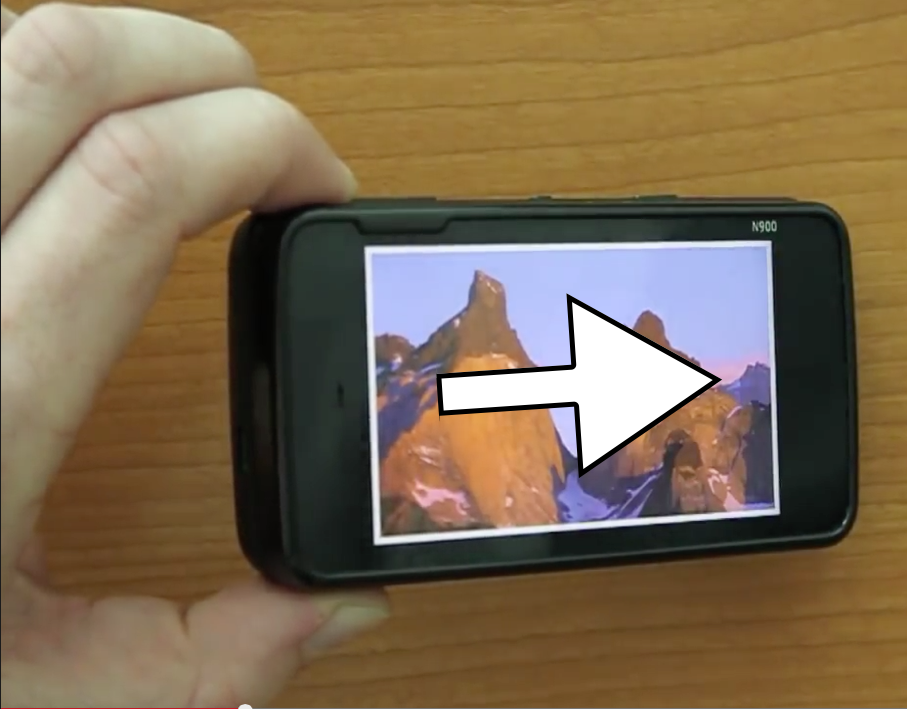
\includegraphics[width=6.5cm]{kapitel2/passThem1.png}
	\caption{Links kippen zum weiterblättern \cite{Lucero:2011:PCU:1978942.1979201}}
	\label{fig:passtThem1}
\end{minipage}
\hfill
\begin{minipage}[h]{7cm}
	\centering
	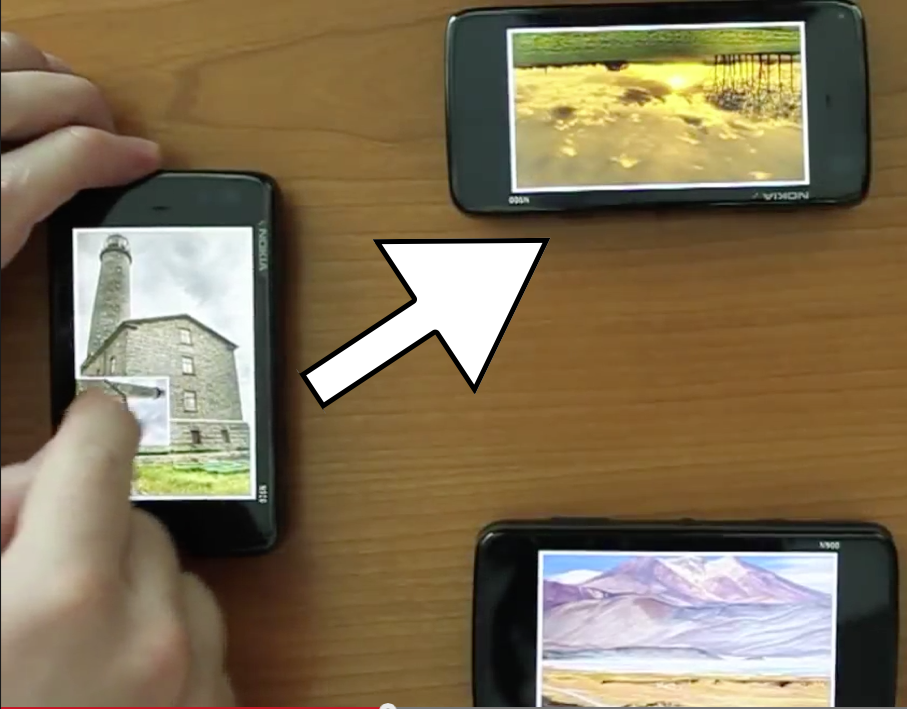
\includegraphics[width=6.5cm]{kapitel2/passThem2.png}
	\caption{Schwung-Geste Auswahl mehrerer Ziele \cite{Lucero:2011:PCU:1978942.1979201}}
	\label{fig:beamTransfer}
\end{minipage}
\end{figure}

\newpage
\section{Technische Grundlagen}
Mobile Endgeräte stecken voller Technologien, um ihre Umwelt wahrzunehmen und mit ihr zu kommunizieren. Dieser Abschnitt identifiziert Technologien zu Datenübertragung, Positionsortung und Sensorik, die für die Implementierung der Bump-Interaktion in Frage kommen.

\subsection{Technologien zur Datenübertragung}

\subsubsection{WLAN}
Ein \ac{WLAN} ist ein lokales Funknetz, das auf der Normenfamilie \acs{IEEE} 802.11 basiert und sich über eine Reichweite von 30 - 100 Meter aufspannen kann. Ein solches Netzwerk kann entweder im Infrastruktur-Modus oder im Ad-hoc-Modus betrieben werden. Der Infrastruktur-Modus ist topologisch wie ein Stern (Siehe Abbildung \ref{fig:topo}) aufgebaut. Endgeräte melden sich an einer zentralen Basisstation an und können danach über diese miteinander kommunizieren. Im Ad-hoc-Modus bauen Endgeräte eine direkte Verbindung miteinander auf ohne den Umweg über eine gesonderte Basistation. Jedes Endgerät kann mehrere Verbindungen zu anderen Geräten unterhalten, womit ein vermaschtes Netzwerk (Siehe Abbildung \ref{fig:topo}) gebildet wird \cite[46-55]{baun2012computernetze}.  

\begin{figure}[H]
\begin{minipage}[h]{7cm}
  \centering
  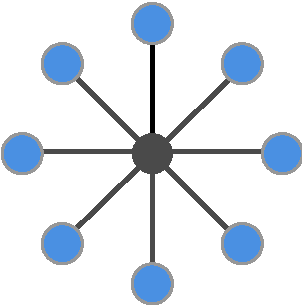
\includegraphics[width=5cm]{kapitel2/SternTopologie.pdf}
  Stern-Topologie
\end{minipage}
\hfill
\begin{minipage}[h]{7cm}
  \centering
  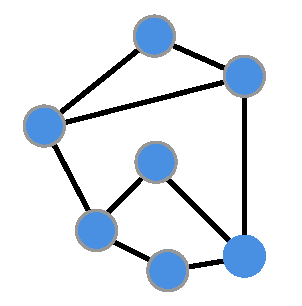
\includegraphics[width=5cm]{kapitel2/MaschenTopologie.pdf}
  Maschentopologie
\end{minipage}
  \caption{WLAN-Topologien \cite[vgl. Abb. 3.1]{baun2012computernetze}}
    \label{fig:topo}
\end{figure}

 Damit Endgeräte verfügbare \ac{WLAN} Netze entdecken können, senden Basistationen oder Ad-hoc Geräte in Intervallen Beacons mit Informationen über das Netzwerk an alle Endgeräte im Empfangsbereich. Sobald Geräte in Reichweite eines Netzwerkes sind, können sie sich direkt verbinden. Sollte das Netzwerk jedoch durch ein Passwort geschützt sein muss dieses erst eingegeben und überprüft werden.
 Es existieren verschiedene \ac{WLAN}-Standards, die sich vor allem durch ihre Datentransferrate unterscheiden. Der weit verbreitete Standard 802.11n bietet im Infrastruktur Modus Übertragungsraten von Brutto 100-120 Mbit/s \cite[46-55]{baun2012computernetze}. Die Geschwindigkeit einer Ad-hoc Verbindungen ist dagegen auf 11 Mbit/s beschränkt \cite{wirtz2011establishing}.

\subsubsection{WIFI-Direct}
WIFI-Direct ist eine spezielle Implementierung des \ac{WLAN} Ad-hoc-Modus. Es liefert signifikant höhere Datenübertragungsraten als der klassische Ad-hoc Modus von bis zu 250 Mbit/s. Für einen einfachen und schnellen Verbindungsaufbau zwischen den Geräten ist es möglich, die Pairing Prozesse von Bluetooth oder \ac{NFC} zu nutzen. WIFI Direct ist verfügbar auf Geräten mit Android oder Windows Betriebssystemen \cite{wiki:WIFI-Direct}.

\subsubsection{Bluetooth Low Energy}
Bluetooth ist ein Funksystem zur Datenübertragung über Distanzen von bis zu 30 Metern \cite{agrawal2012near}. Ab der Version 4.0 spricht man auch von Bluetooth Low Energy, da ab dieser Version die Technologie auf sehr niedrigen Stromverbrauch optimiert wurde. Um miteinander zu kommunizieren, bauen Endgeräte eine Peer to Peer Verbindung untereinander auf und organisieren sich in sogenannten Pico Netzen (Siehe Abbildung \ref{fig:pico1}). Ein Pico Netz besteht aus maximal 255 Teilnehmern wovon maximal acht aktiv sein dürfen. Einer der aktiven Teilnehmer nimmt dabei die Rolle des Masters ein, während die anderen sieben Slaves sind. Die restlichen 247 Teilnehmer sind passiv, können jedoch jederzeit vom Master aktiviert werden. Der Master steuert die Kommunikation und den Datenverkehr zwischen den Teilnehmern des Netzes \cite[55-57]{baun2012computernetze}. 

\begin{figure}[H]
\begin{minipage}[hbt]{7cm}
  \centering
  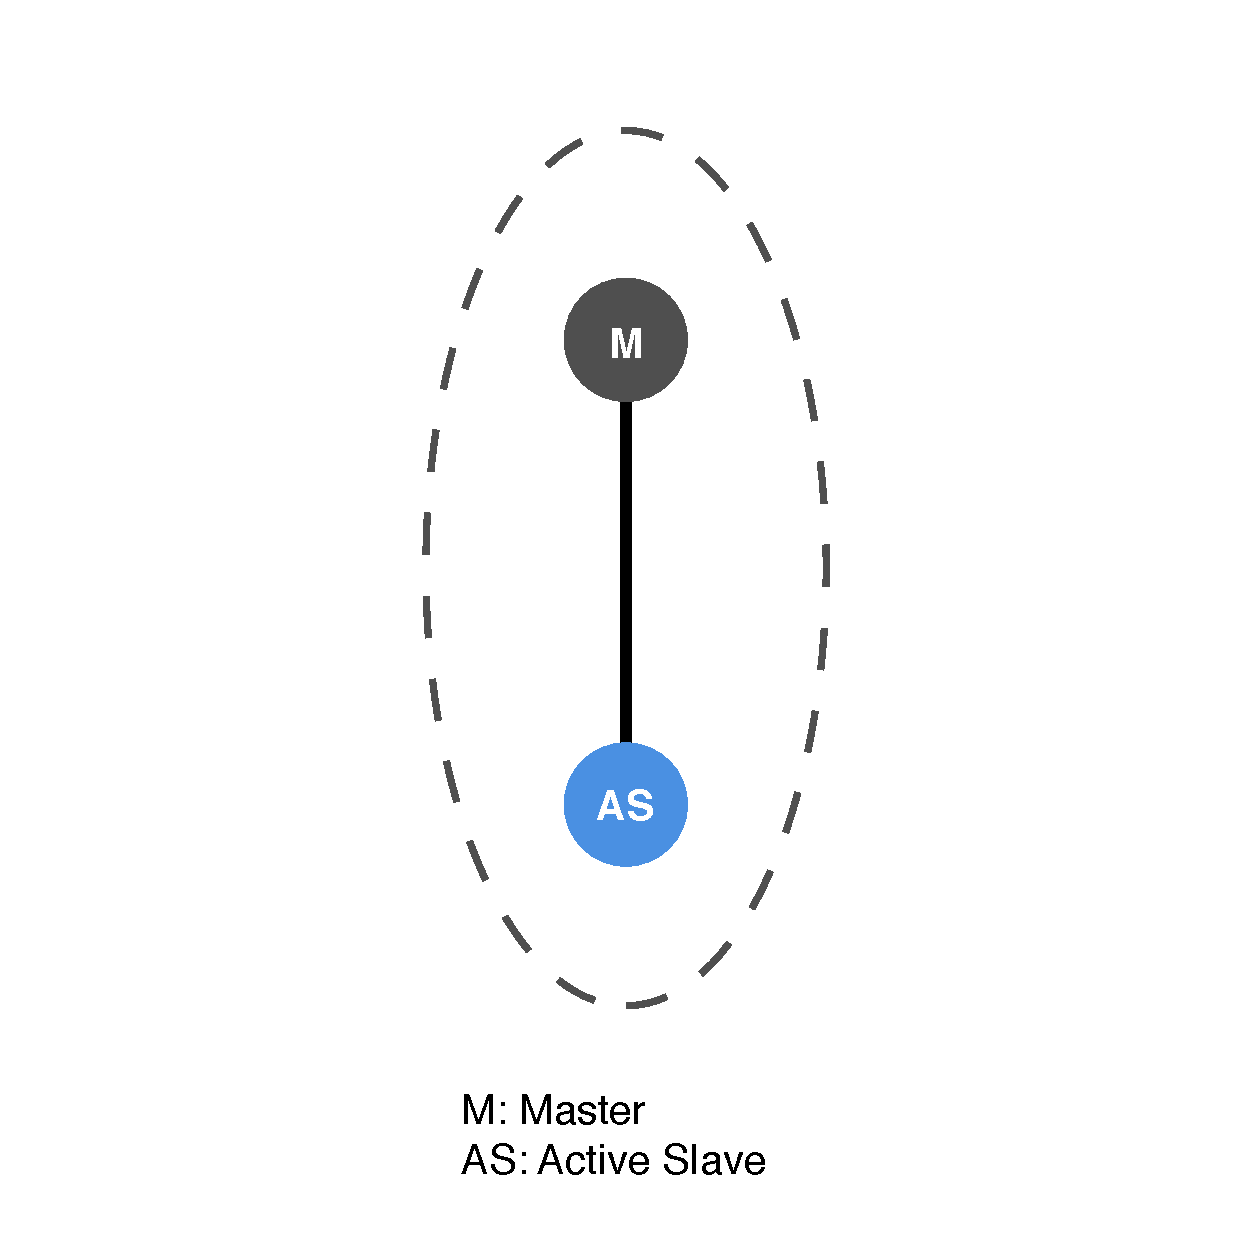
\includegraphics[width=7cm]{kapitel2/PicoNetz1.pdf}
\end{minipage}
\hfill
\begin{minipage}[hbt]{7cm}
  \centering
  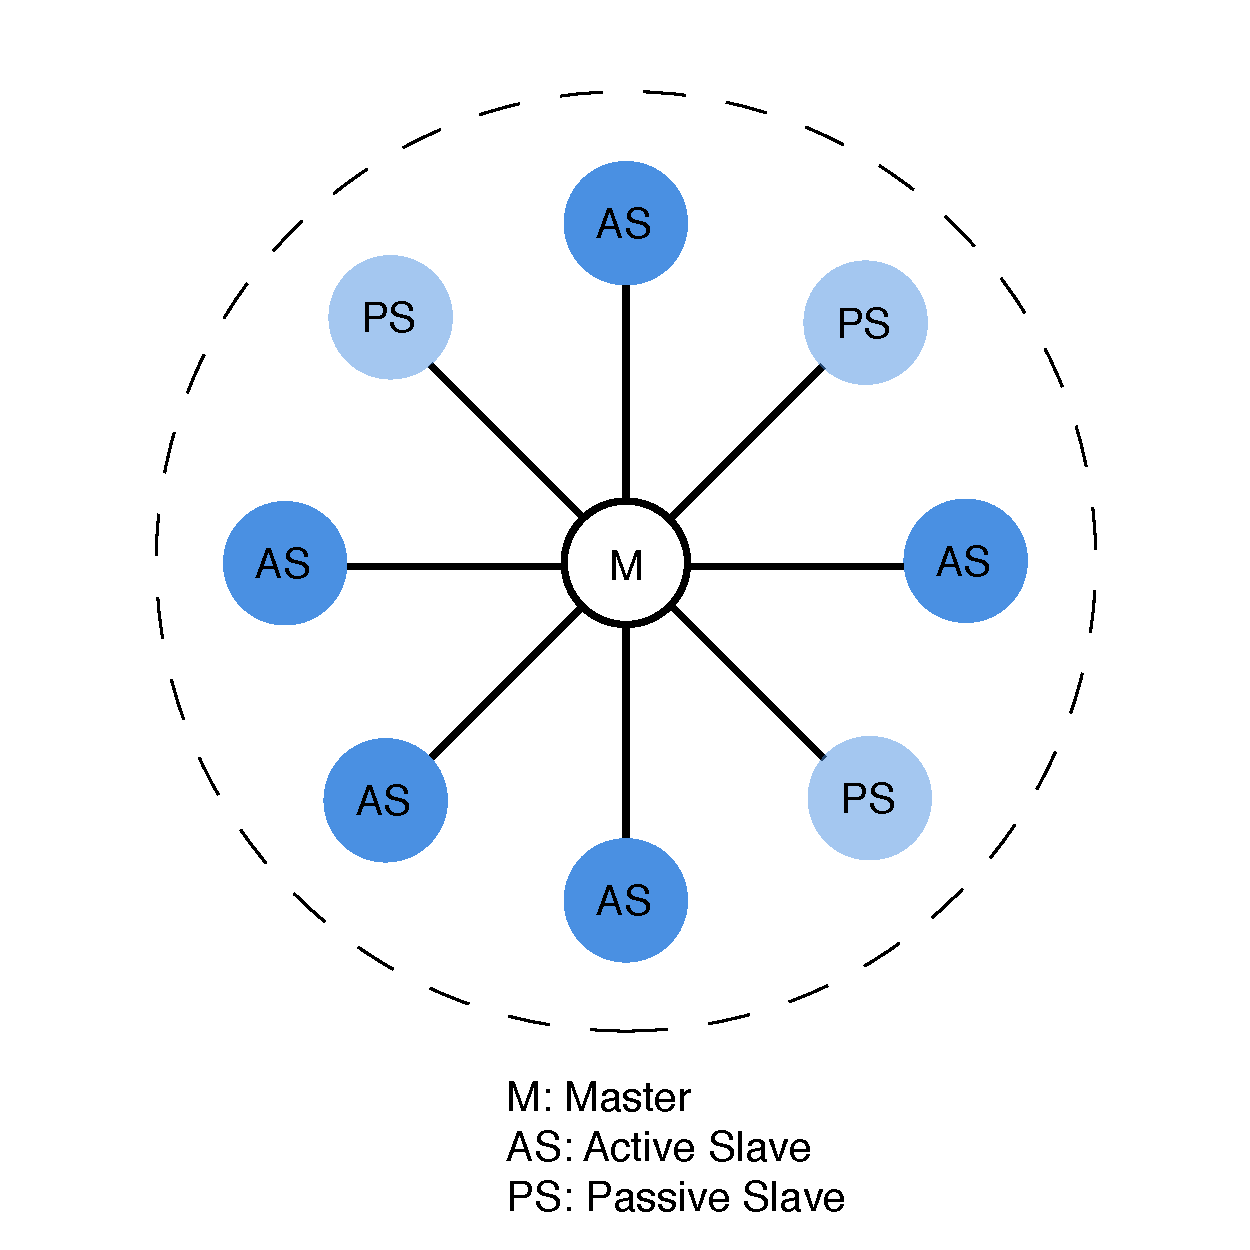
\includegraphics[width=7cm]{kapitel2/PicoNetz2.pdf}
\end{minipage}
\caption{Bluetooth-Topologie Piconetz \cite[vgl. Abb. 5.4]{baun2012computernetze}}
\label{fig:pico1}
\end{figure}

Bevor Daten übertragen werden können, müssen sich Geräte erst über den Vorgang des Pairings kennen lernen. Bei diesem Vorgang müssen die Benutzer jeweils einen gemeinsamen Code durch Tastendruck auf ihrem Gerät bestätigen. Nachdem Geräte einmal gepaired wurden, ist ein weiteres Pairing nicht mehr nötig, da sie sich bereits kennen. Seit Version 3.0 beherrscht Bluetooth den High Speed Modus, welcher eine Kombination aus Bluetooth und \ac{WLAN} 802.11g ist. Über die Bluetooth Verbindung mit 3 Mbit/s werden dabei nur noch Steuerdaten sowie Sitzungsschlüssel übertragen. Für die Nutzdaten wird eine Ad-hoc Verbindung über \ac{WLAN} aufgebaut, die eine Datentransferrate von ca 24 Mbit/s erreicht \cite[55-57]{baun2012computernetze}.

\subsubsection{NFC} 
Near Field Communication auch als \ac{NFC} bekannt, ist eine Funktechnologie für sehr kurze Distanzen. In einer Reichweite von optimal 4 cm und maximal  20 cm können Geräte miteinander eine Peer to Peer Verbindung eingehen und Daten mit bis zu 424 kBit/s übertragen. Anders als bei \ac{WLAN} und Bluetooth ist es mit \ac{NFC} nicht möglich, Verbindungen zu mehreren Geräten gleichzeitig zu unterhalten. Einen weiteren Unterschied stellt der Verbindungsaufbau zwischen den Geräten dar. Dieser ist bei \ac{NFC} sehr einfach gestaltet, da das Pairing allein durch die unmittelbare Nähe der Geräte zueinander geschieht und keine weiteren Aktionen des Nutzers benötigt. Aus diesem Grund wird \ac{NFC} auch in Verbindung mit Bluetooth oder \ac{WLAN} genutzt um schnell und einfach eine Verbindung aufzubauen ohne Passworteingabe bei \ac{WLAN} oder Code Bestätigung bei Bluetooth \cite{agrawal2012near}. \ac{NFC} ist verfügbar auf Android- und Windows-Geräten. Obwohl \ac{NFC} ab dem iPhone 6 integriert ist, sind keine \acs{API}s für Entwickler vorhanden. 

\subsubsection{Mobilfunk}
Moderne Mobilfunknetze bieten neben dem Zugang zu Telefondiensten auch Zugang zu Internetdiensten. Die aktuellsten Mobilfunkstandards sind \ac{HDSPA+} und \ac{LTE}. Bei \ac{HDSPA+} handelt es sich um eine Erweiterung des Mobilfunkstandards \acs{UMTS} mit Datenraten von bis zu 42 Mbit/s \cite{HDSPA:Online}. \ac{LTE} dagegen ist eine komplett neu entwickeltes Mobilfunknetz, das in der aktuellen Spezifikation theoretische Datenraten von bis zu 75 Mbit/s im Upload und 300 Mbit/s im Download bietet \cite{LTE:Online}.

\subsection{Datenkommunikation zwischen mobilen Endgeräten}
Über die Technologien, die im vorherigen Abschnitt beschrieben wurden, kann abhängig von der Technologie, entweder direkt zwischen Geräten im Netzwerk oder über einen Server kommuniziert werden. Folgend wird beschrieben, mit welchen Protokollen die Kommunikation in beiden Fällen umgesetzt werden kann. 

\subsubsection{Datenkommunikation in lokalen Netzwerken}
Sollen mobile Applikationen über ein lokales Netzwerk miteinander kommunizieren kann dies durch die Nutzung von Netzwerkdiensten realisiert werden. Ein Netzwerkdienst ist ein Informationsobjekt, das von einer Person, einem Programm, oder von einem anderen Dienst genutzt werden kann. Jeder Dienst stellt eine Funktionalität zur Verfügung, dabei kann es sich z.B. um Anwendungsdienste oder Kommunikationsdienste handeln \cite{cheng2002service}.  Eine wichtige Komponente zur Nutzung von Diensten ist \textit{service discovery}, über welches angebotene Dienste in einem Netzwerk gefunden werden können. Für service discovery existieren verschiedene Protokolle. Apple nutzt in seinen Betriebssystemen Bonjour \cite{AboutBonjour:Online}, Android nutzt Network Service Discovery \cite{AndroidDiscovery:Online}, um nur zwei Vertreter zu nennen. Beide Protokolle ermöglichen das automatische entdecken von Geräten und Diensten in lokalen Netzwerken.

Ein Dienst wird unter Anderem durch seinen Namen beschrieben. Dieser Name ist im Netzwerk sichtbar für alle Geräte, die danach suchen. Angebotene Dienste sollten einen einzigartigen Namen aufweisen, um Konflikte zwischen verschiedenen Applikationen zu vermeiden. Durch den Einsatz von Diensten können verschiedene Applikationen in einem Netzwerk untereinander kommunizieren. Dabei ist die Topologie des Netzwerkes unerheblich. Netzwerkdienste können in Infrastrukturnetzwerken (Siehe Abbildung \ref{fig:diensteGrund} a) genutzt werden und auch um Ad-Hoc Netzwerke zu bilden (Siehe Abbildung \ref{fig:diensteGrund} b).

\begin{figure}[H]
  \centering
  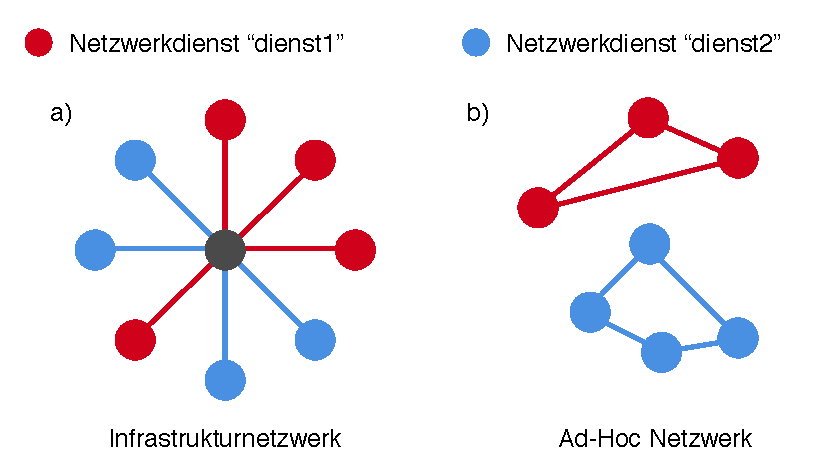
\includegraphics[width=\linewidth]{kapitel2/netzwerkdiensteGrundlagen.pdf}
  \caption{Netzwerkdienste in Computernetzwerken}
  \label{fig:diensteGrund}
\end{figure}

\subsubsection{Datenkommunikation über einen Server}
Anstatt direkt in einem lokalen Netzwerk zu kommunizieren, können Applikationen auch über einen Server Daten austauschen. Das Standardmodell für diese Kommunikation ist das Client-Server-Modell (Siehe Abbildung \ref{fig:clientServer}). In diesem Modell rufen Clients bestimmte Funktionalitäten bzw. Dienstleistungen, die ein Server zur Verfügung stellt, über ein Netzwerk hinweg auf \cite[14]{schill2012verteilte}.  
\begin{figure}[H]
  \centering
  \includegraphics[width=10cm]{kapitel2/clientServer.pdf}
  \caption{Client-Server-Modell}
  \label{fig:clientServer}
\end{figure}
\subsubsection{HTTP Operationen}
Clients stehen \acs{HTTP} Operationen zur Verfügung, mit denen die Kommunikation mit einem Server erfolgen kann. Die wichtigsten dieser Operationen \cite[14]{rodriguez2008restful}, sind die sogenannten \acs{CRUD} Operationen: create, read, update and delete. Die entsprechenden \acs{HTTP} Methoden, mit denen diese Operationen durchgeführt werden können, sind:
\begin{itemize}
\item POST um Ressourcen auf dem Server anzulegen.
\item GET um Ressourcen aufzurufen.
\item PUT um eine Recource zu aktualisieren
\item DELETE um eine Recource zu löschen
\end{itemize}
Endgeräte tauschen über diese Methoden Daten aus, indem eines der Geräte eine Ressource auf dem Server anlegt, während das andere Gerät die entsprechende Ressource aufruft. Der Datenaustausch über diese Methoden hat zur Folge, dass Clients anhaltend überprüfen müssen, ob die Daten bereits auf dem Server verfügbar sind. Für mobile Endgeräte ist dieser Vorgang aber nachteilig, da die ständigen Anfragen an den Server kostbare Batterielaufzeit verschwenden \cite{lando2007efficient}. Es existiert jedoch eine alternative Möglichkeit, mit der Client und Server kommunizieren können ohne dieses Problem, in der Form von Web Sockets.

\subsubsection{Web Sockets}
Web Sockets ermöglichen eine bidirektionale Verbindung zwischen einer Anwendung und einem Webserver. Wurde einmal eine Socket Verbindung durch den Client geöffnet, kann diese Verbindung aus beiden Richtungen verwendet werden. Für einen Datenaustausch bedeutet dies, dass Endgeräte nicht konstant nachfragen müssen, ob eine Ressource vorhanden ist. Der Server sendet die Daten selbstständig an die Clients, sobald Sie verfügbar sind. Socket-Verbindungen bleiben dauerhaft bestehen und werden erst geschlossen, wenn der Client die Verbindung schließt \cite{lubbers2010html5}.



\subsection{Technologien zur Geräteortung}

\subsubsection{GPS}
\label{subsec:GPS}
Das Global Positioning System \ac{GPS} ist ein globales mit Satelliten betriebenes Navigationssystem zur Positionsbestimmung. Ist ein Endgerät mit \ac{GPS} ausgestattet, ist es möglich, den Standort dieses Geräts zu bestimmen. Der Standort wird in geographische Koordinaten angegeben, mit denen sich die Lage eines Punktes auf der Erde beschreiben lässt \cite{wiki:GPS}. Die Funktionsfähigkeit von \ac{GPS} ist maßgeblich von der Empfangsqualität abhängig, so ist eine Ortung in Gebäuden häufig nicht möglich und auch die Genauigkeit der Positionsbestimmung kann negativ beeinflusst werden. In der Regel wird \ac{GPS} in Kombination mit anderen Technologien wie Mobilfunk-, \ac{WLAN}- oder Bluetooth genutzt. Dadurch kann zum einen der Verbindungsaufbau zu den Satelliten beschleunigt und zum anderen die Genauigkeit der Standortbestimmung verbessert werden. Trotz dieser Technik unterliegen die mit \ac{GPS} ermittelten Standortdaten häufig einer Ungenauigkeit die mehrere Meter hoch ausfallen kann \cite{AppleLocationServices:Online}.

\subsubsection{iBeacon}
\label{subsec:beacons}
Mit iBeacon können standortbezogene Dienste und Navigationslösungen in geschlossenen Räumen realisiert werden. iBeacon ist Apple's Markenname für eine Technologie, die Teil des Bluetooth Low Energy Standards ist. Dadurch ist iBeacon auf allen Endgeräten verfügbar die über Bluetooth LE verfügen und deren Betriebssystem kompatibel ist. Momentan sind das \acs{iOS}7 und Android 4.3. Neben Software Komponenten umfasst die Beacon Technologie auch Hardware Komponenten. Dies sind speziell entwickelte Signalgeber, ebenfalls als iBeacons oder Beacons bezeichnet, die mit Bluetooth LE Technik ausgestattet sind. Diese Hardware Beacons werden jedoch nicht in allen Anwendungsszenarien benötigt, da jedes kompatible Smartphone ebenfalls die Funktionen eines Beacons übernehmen kann \cite{wiki:iBeacon}.

iBeacon unterscheidet drei Grundlegende Funktionen: \textit{Advertising}, \textit{Ranging} und \textit{Region Monitoring}. Im folgenden werden diese Funktionen beschrieben und die Funktionsweise der Beacon Technologie dargestellt.

\paragraph{Advertising}
ist der Vorgang mit dem Beacons andere Geräte über ihre Anwesenheit informieren. Jedes Beacon spannt einen Bereich um sich, der als \textit{region} bezeichnet wird. Innerhalb dieses Aktionsradius senden Beacons kontinuierlich Signale mit Informationen über ihre Identität aus.

Die Identität eines Beacons setzt sich zusammen aus einer 16 Byte \textit{\acs{UUID}} (\acl{UUID}) sowie einem \textit{major} und einem \textit{minor} Wert die jeweils 2 Byte groß sind. Die \textit{\acs{UUID}} ist ein Identifikator der je nach Anwendungsfall von einem oder mehreren Beacons genutzt werden kann. Mit \textit{major} und \textit{minor} Wert kann für jedes Beacon eine einzigartige ID gebildet werden mit der dieses eindeutig aus einer Gruppe von Beacons mit der selben \textit{\acs{UUID}} identifiziert werden kann (Siehe Abbildung \ref{fig:beaconRegion}).

\begin{figure}[H] 
\centering 
  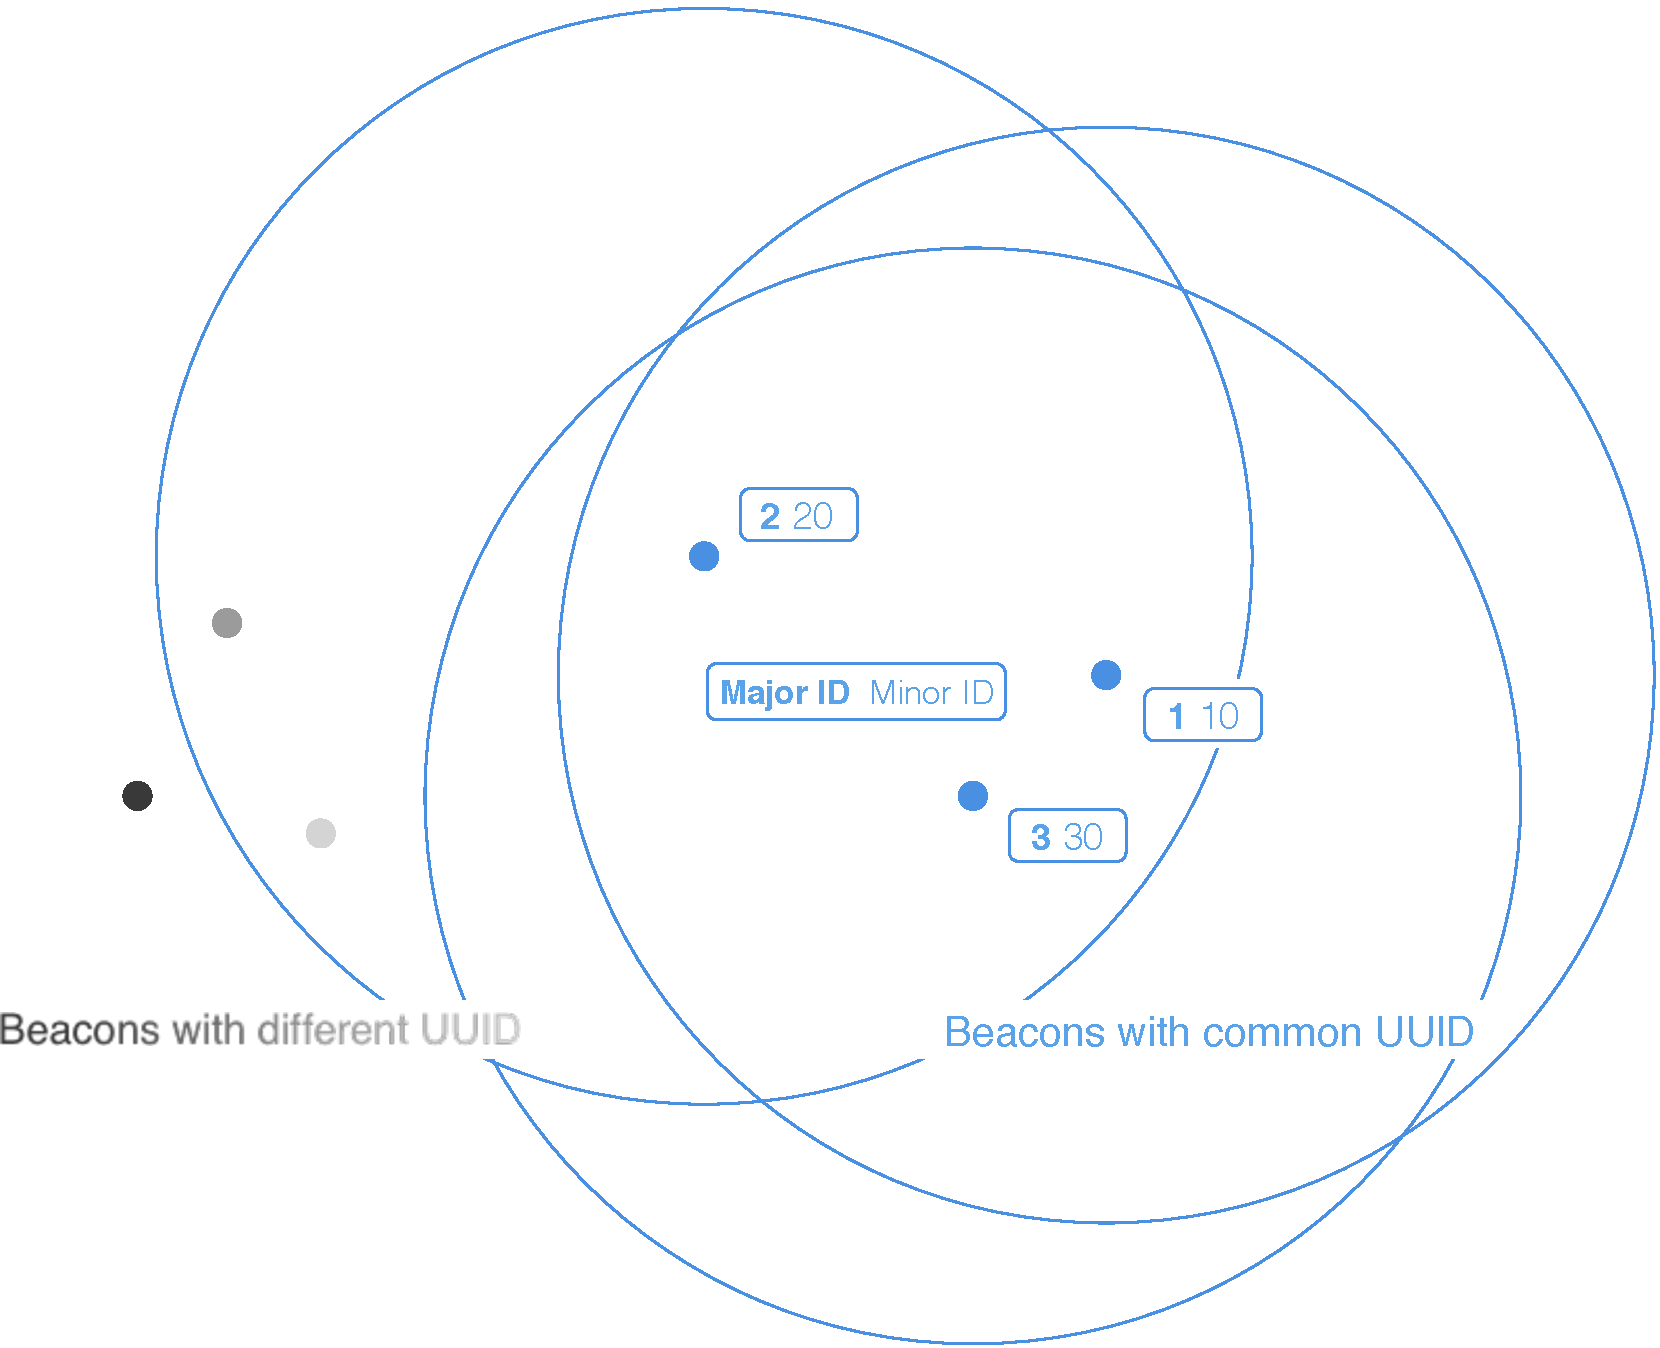
\includegraphics[width=\linewidth]{kapitel2/beaconRegions.pdf}
  \caption{iBeacon regions}
  \label{fig:beaconRegion}
\end{figure}

Die folgende Tabelle zeigt ein Beispiel wie die Werte genutzt werden können um iBeacons in einer Einzelhandelskette einzusetzen.

\begin{table}[H]
\centering
\begin{tabular}{| >{\centering\arraybackslash}m{1.5cm} | >{\centering\arraybackslash}m{2cm} | >{\centering\arraybackslash}m{2,8cm} | >{\centering\arraybackslash}m{2,8cm} | >{\centering\arraybackslash}m{2,8cm} |}
\hline
\multicolumn{2}{|c|}{\cellcolor[HTML]{C0C0C0}Store Location}  & \cellcolor[HTML]{C0C0C0}San Francisco & \cellcolor[HTML]{C0C0C0}Paris & \cellcolor[HTML]{C0C0C0}London\\
\hline
\multicolumn{2}{|c|}{\cellcolor[HTML]{EFEFEF}UUID}  & \multicolumn{3}{c|}{D9B9EC1F-3925-43D0-80A9-1E39D4CEA95C}\\
\hline
\multicolumn{2}{|c|}{\cellcolor[HTML]{EFEFEF}Major} & 1 & 2 & 3\\
\hline
\cellcolor[HTML]{EFEFEF} & \cellcolor[HTML]{EFEFEF}Clothing & 10 & 10 & 10\\
\cline{2-5}
\cellcolor[HTML]{EFEFEF}Minor & \cellcolor[HTML]{EFEFEF}Housewares & 20 & 20 & 20\\
\cline{2-5}
\cellcolor[HTML]{EFEFEF} & \cellcolor[HTML]{EFEFEF}Automotive & 30 & 30 & 30\\
\hline
\end{tabular}
\caption{Einsatz von Beacons in einer Einzelhandelskette \cite{iBeacon:2014}}
\label{tableBeacon}
\end{table}

In diesem Beispiel wird die \textit{\acs{UUID}} von den Beacons an allen Standorten gemeinsam genutzt und Identifiziert die Handelskette als ganzes. Jede Filiale wird durch einen \textit{major} Wert identifiziert. Innerhalb einer jeden Filiale werden die einzelnen Abteilungen durch einen \textit{minor} Wert repräsentiert. Mit Hilfe dieser Informationen ist eine Applikation in der Lage festzustellen, ob der Benutzer eine der Filialen betritt, verlässt und in welcher Abteilung er sich gerade befindet \cite{iBeacon:2014}.

\paragraph{Ranging}
ist die Funktion mit der eine Applikation nach Signalen sucht die von Beacons ausgesendet werden. Es können dabei nur Signale empfangen werden von Beacons deren \textit{\acs{UUID}} der Applikation bekannt sind. Werden zum ersten mal Signale eines solchen Beacons empfangen, wurde die \textit{region} dieses Beacons betreten und ein Event wird in der Applikation ausgelöst. Umgekehrt bedeutet der langfristige Verlust des Beacon-Signals, dass die \textit{region} verlassen wurde. Wie beim Betreten, wird auch beim Verlassen einer \textit{region} ein entsprechendes Event in der Applikation ausgelöst \cite{iBeacon:2014}.

Nachdem eine \textit{region} betreten wurde, kann der Abstand zum Beacon anhand der Signalstärke \textit{\acs{RSSI}} (\acl{RSSI}) näherungsweise bestimmt werden. Die Ermittlung des Abstands ist anfällig, ungenaue Ergebnisse zu produzieren da das Signal durch externe Faktoren beeinflusst werden kann \cite{EstimoteBeaconSignal:Online}. Bei diesen Faktoren kann es sich sowohl um Räumliche Begebenheiten handeln als auch um Interferenzen die durch andere Funksignale z.B. durch WLAN ausgelöst werden können. Der iBeacon Hersteller Estimote ermittelte in internen Tests Abweichungen von 5-6cm bei einem Abstand von 20cm sowie 2-3m bei Abständen von über 10m \cite{EstimoteBeaconSignal:Online}. Die Genauigkeit der Messung scheint also fundamental vom Abstand zu Beacons bzw.  der Signalstärke abzuhängen. Um Entwicklern eine Möglichkeit zu geben, auf Ungenaue Messergebnisse zu reagieren, gibt \acs{iOS} eine Einschätzung zur Genauigkeit der Messung mit dem \textit{accuracy} Parameter aus. Ist der \textit{accuracy} Wert niedrig bedeutet dies, dass sich \acs{iOS} sehr sicher ist über die Genauigkeit der Messung. Umgekehrt bedeutet ein hoher \textit{accuracy} Wert, dass der ermittelte Abstand sehr wahrscheinlich ungenau ist \cite{iBeacon:2014}.

Ist für ein Anwendungsszenario eine ungefähre Abschätzung über den Abstand zu einem Beacon ausreichend, kann man diese über die vier vordefinierten \textit{proximity states} erhalten. Diese lauten: \textit{unknown}, \textit{far}, \textit{near} und \textit{immediate}. \textit{Unknown} beschreibt dabei die Entfernung, die ermittelt wird, sollte sich das Smartphone außerhalb der Reichweite des Beacons befinden oder sollte die Qualität der empfangenen Signale nicht ausreichen, um den Abstand festzustellen. Wird \textit{far} als Abstand ausgegeben, werden Beacon Signale empfangen, jedoch sind Sie schwach oder \acs{iOS} ist sich unsicher über die Genauigkeit der Messung. Der Abstand zum Beacon kann zwischen 70m und 3m liegen. \textit{near} beschreibt eine Zone in der die Signalstärke gut ist und die Genauigkeit ebenfalls als gut eingeschätzt wird. Der Abstand zum Beacon bewegt sich zwischen 0.5m und 3m. Der letzte mögliche \textit{proximity state} ist \textit{immediate}. Wird dieser Status angezeigt ist die Signalstärke sehr hoch und \acs{iOS} ist sich sehr sicher über die Genauigkeit der Messung. Der Empfänger befindet sich in einem Abstand von unter 0.5m zum Sender (Siehe Abbildung \ref{fig:beaconRegion}). In einer Applikation wird für jeden der \textit{proximity state} ein entsprechendes Event ausgelöst sobald dieser festgestellt wird \cite{EstimoteBeaconSignal:Online}.

\begin{figure}[H] 
\centering 
  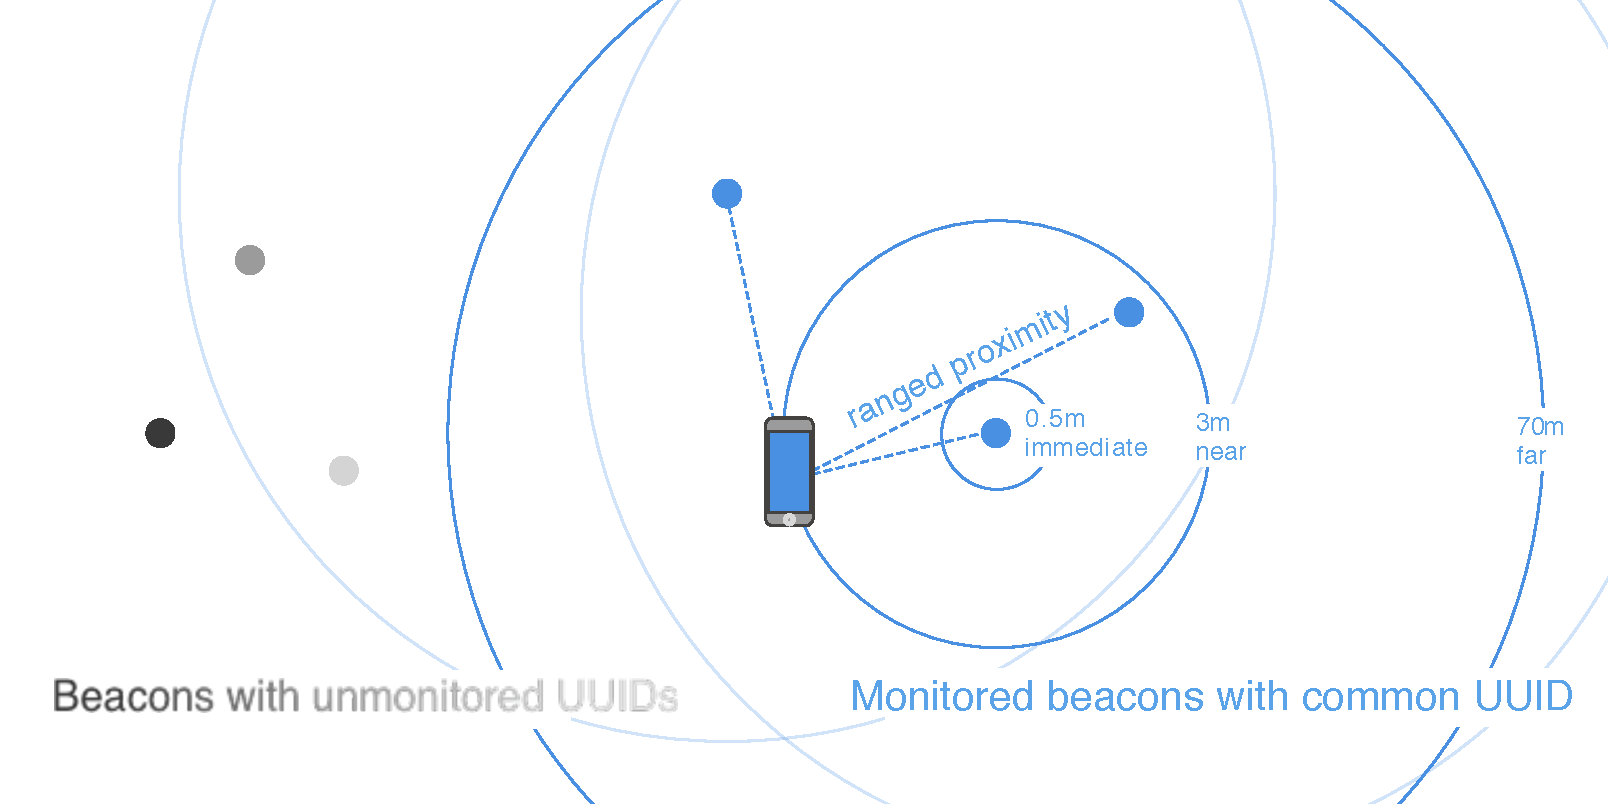
\includegraphics[width=\linewidth]{kapitel2/beaconRanging.pdf}
\caption{iBeacon ranging} 
\end{figure}

\paragraph{Region Monitoring} bietet eine weitere Funktionalität mit der Applikationen Events auslösen können sobald das Smartphone eine definierte Beacon \textit{region} betritt oder verlässt. Dafür muss die Bump-Applikation im Gegensatz zur selben Funktionalität beim \textit{Ranging} nicht aktiv sein. Geschlossene Applikationen können durch das \textit{Region Monitoring} im Hintergrund gestartet werden und z.B. \textit{Push Notifications} auslösen. Andere Aktionen die ausgeführt werden können, während eine Applikation im Hintergrund ist, sind auch möglich.

\subsection{Sensoren}
Mobile Endgeräte sind mit einer Reihe von Sensoren ausgestattet, mit denen es möglich ist, unentwegt Daten zu sammeln. Applikationen können diese Daten auswerten, um zu sehen, hören und fühlen, was mit dem Gerät und in seiner Umgebung geschieht. Bewegungen des Anwenders bzw. des Endgeräts können durch die Auswertung der Daten des Beschleunigungssensors erkannt werden. Ein Beschleunigungssensor, auch Accelerometer genannt, ist ein Sensor, mit dem Beschleunigung oder g-Kraft in Meter pro Quadratsekunde ($m/m^{2}$) gemessen werden kann. In mobilen Endgeräten sind in der Regel drei Sensoren eingebaut, mit denen die Beschleunigung auf x, y und z-Achse bestimmt werden kann (Siehe Abbildung \ref{fig:Beschleunigungssensor}). Durch die Auswertung der Sensordaten können Bewegungen des Benutzers z.B. laufen, rennen oder Treppensteigen erkannt werden. Die Daten können aber auch genutzt werden, um zu erkennen, ob sich ein Endgerät im freien Fall befindet, oder um Erschütterungen festzustellen, wenn das Gerät gegen etwas stößt \cite{ravi2005activity}. 

\begin{figure}[H]
    \centering
    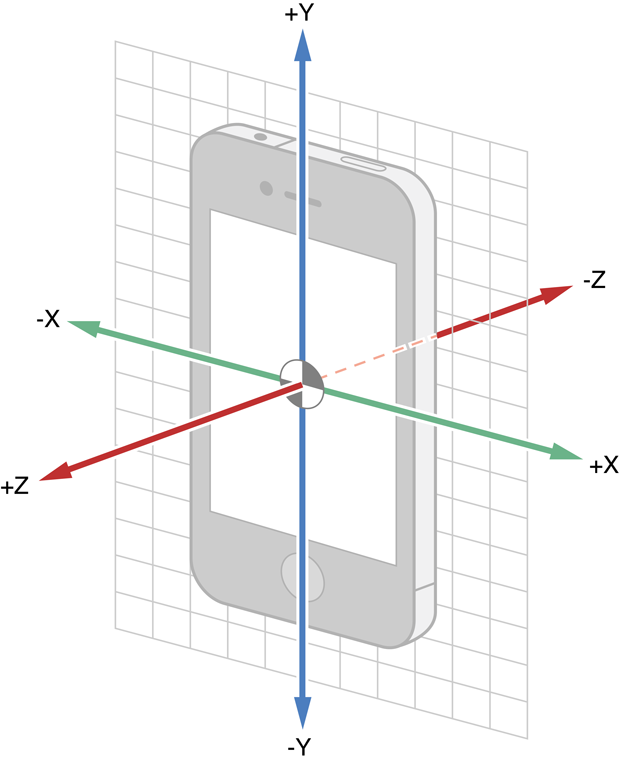
\includegraphics[width=0.4\textwidth]{kapitel2/Accelerometer.png}
    \caption{3-Achsen Beschleunigugnssensor \cite{AppleAccelerometer:Online}}
    \label{fig:Beschleunigungssensor}
\end{figure}